\documentclass{article}
\usepackage{amsmath}
\usepackage{braket}
\usepackage{amssymb}
\usepackage{hyperref}
\usepackage{booktabs}
\usepackage{graphicx}
\newcommand{\bfit}[1]{\textit{\textbf{#1}}}
\begin{document}
\textbf{\Large Chapter 10\\
Spin Qubit-Rabi Oscillation Under Rotating Field Using Rotating Frame}\\\\\\
\textbf{\large 10.1 Introduction}\\\\
We learned the physics and mathematics of Rabi oscillation due to a perturbating linearly
oscillating magnetic field in the previous chapter (Fig.9.2). The skills and insights
we gained are important. However, the mathematics used was cumbersome.
The freedom of applying a linearly oscillating magnetic field to construct a quantum
gate is also limited. In this chapter, we will consider a magnetic field rotation on the
$\hat{x}-\hat{y}$ plane. It gives a great degree of freedom to rotate a state on the Bloch
sphere about any axis (not just the axis along the oscillating field as in the linear case).
Moreover, the magentic field magnitude need not be small.\\\\\\
\bfit{\large 10.1.1 Leraning Outcomes}\\\\
Understand the difference between applying a linearly oscillating magnetic field and applying
a rotating magnetic field; be able to solve the Schr\"{o}dinger equation in the rotating frame.\\\\\\
\bfit{\large 10.1.2 Teaching Videos}\\\\
$\bullet$ Search for Ch10 in this playlist\\

- \url{https://tinyurl.com/3yhze3jn}\\\\
$\bullet$ Other videos\\

- \url{https://youtu.be/cPqby7gujFc}\\

- \url{https://youtu.be/r9wmOw3uxzk}\\\\\\
\textbf{\large 10.2 Experimental Setup}\\\\
The experimental setup is shown in Fig. 10.1. Besides the vertical DC magnetic
field, $\vec{B}=-B_0\hat{z}$ with $B_0>0$, it also has a rotating magnetic field on the 
$\hat{x}-\hat{y}$ plane. This field rotates about the origin at an angular frequency
of  $\omega_1$. Note that we sest it so that it is rotating in the same direction (clockwise
seen from the top) as the Larmor precession. It has the following expression:
\begin{equation}\label{eq 10.1}
    \vec{B_\bot}=B_\bot(\cos(\omega_1t+\phi_B)\hat{x}-\sin(\omega_1t+\phi_B)\hat{y}).\tag{10.1}
\end{equation}
where the initial phase of the field is $\phi_B$. Its amplitude is $B_\bot$ (we do $NOT$ assume it
to be much smaller than $B_0$). Later we will see both $\phi_B$ and $B_\bot$ play
an important role in controlling qubit state rotation and, thus, determine the qubit gate it will 
construct.

The total magnetic field is thus given by,
\begin{align*}\label{eq 10.2}
    \vec{B_\bot}&=\vec{B_\bot}-B_0\hat{z},\\
    &=B_\bot(\cos(\omega_1t+\phi_B)\hat{x}-\sin(\omega_1t+\phi_B)\hat{y})-B_0\hat{z},\\
    &=\begin{pmatrix}
        B_\bot\cos(\omega_1t+\phi_B)\\
        -B_\bot\sin(\omega_1t+\phi_B)\\ -B_0
    \end{pmatrix}.\tag{10.2}
\end{align*}
where we write it in a 3D vector column form in the last line.\\

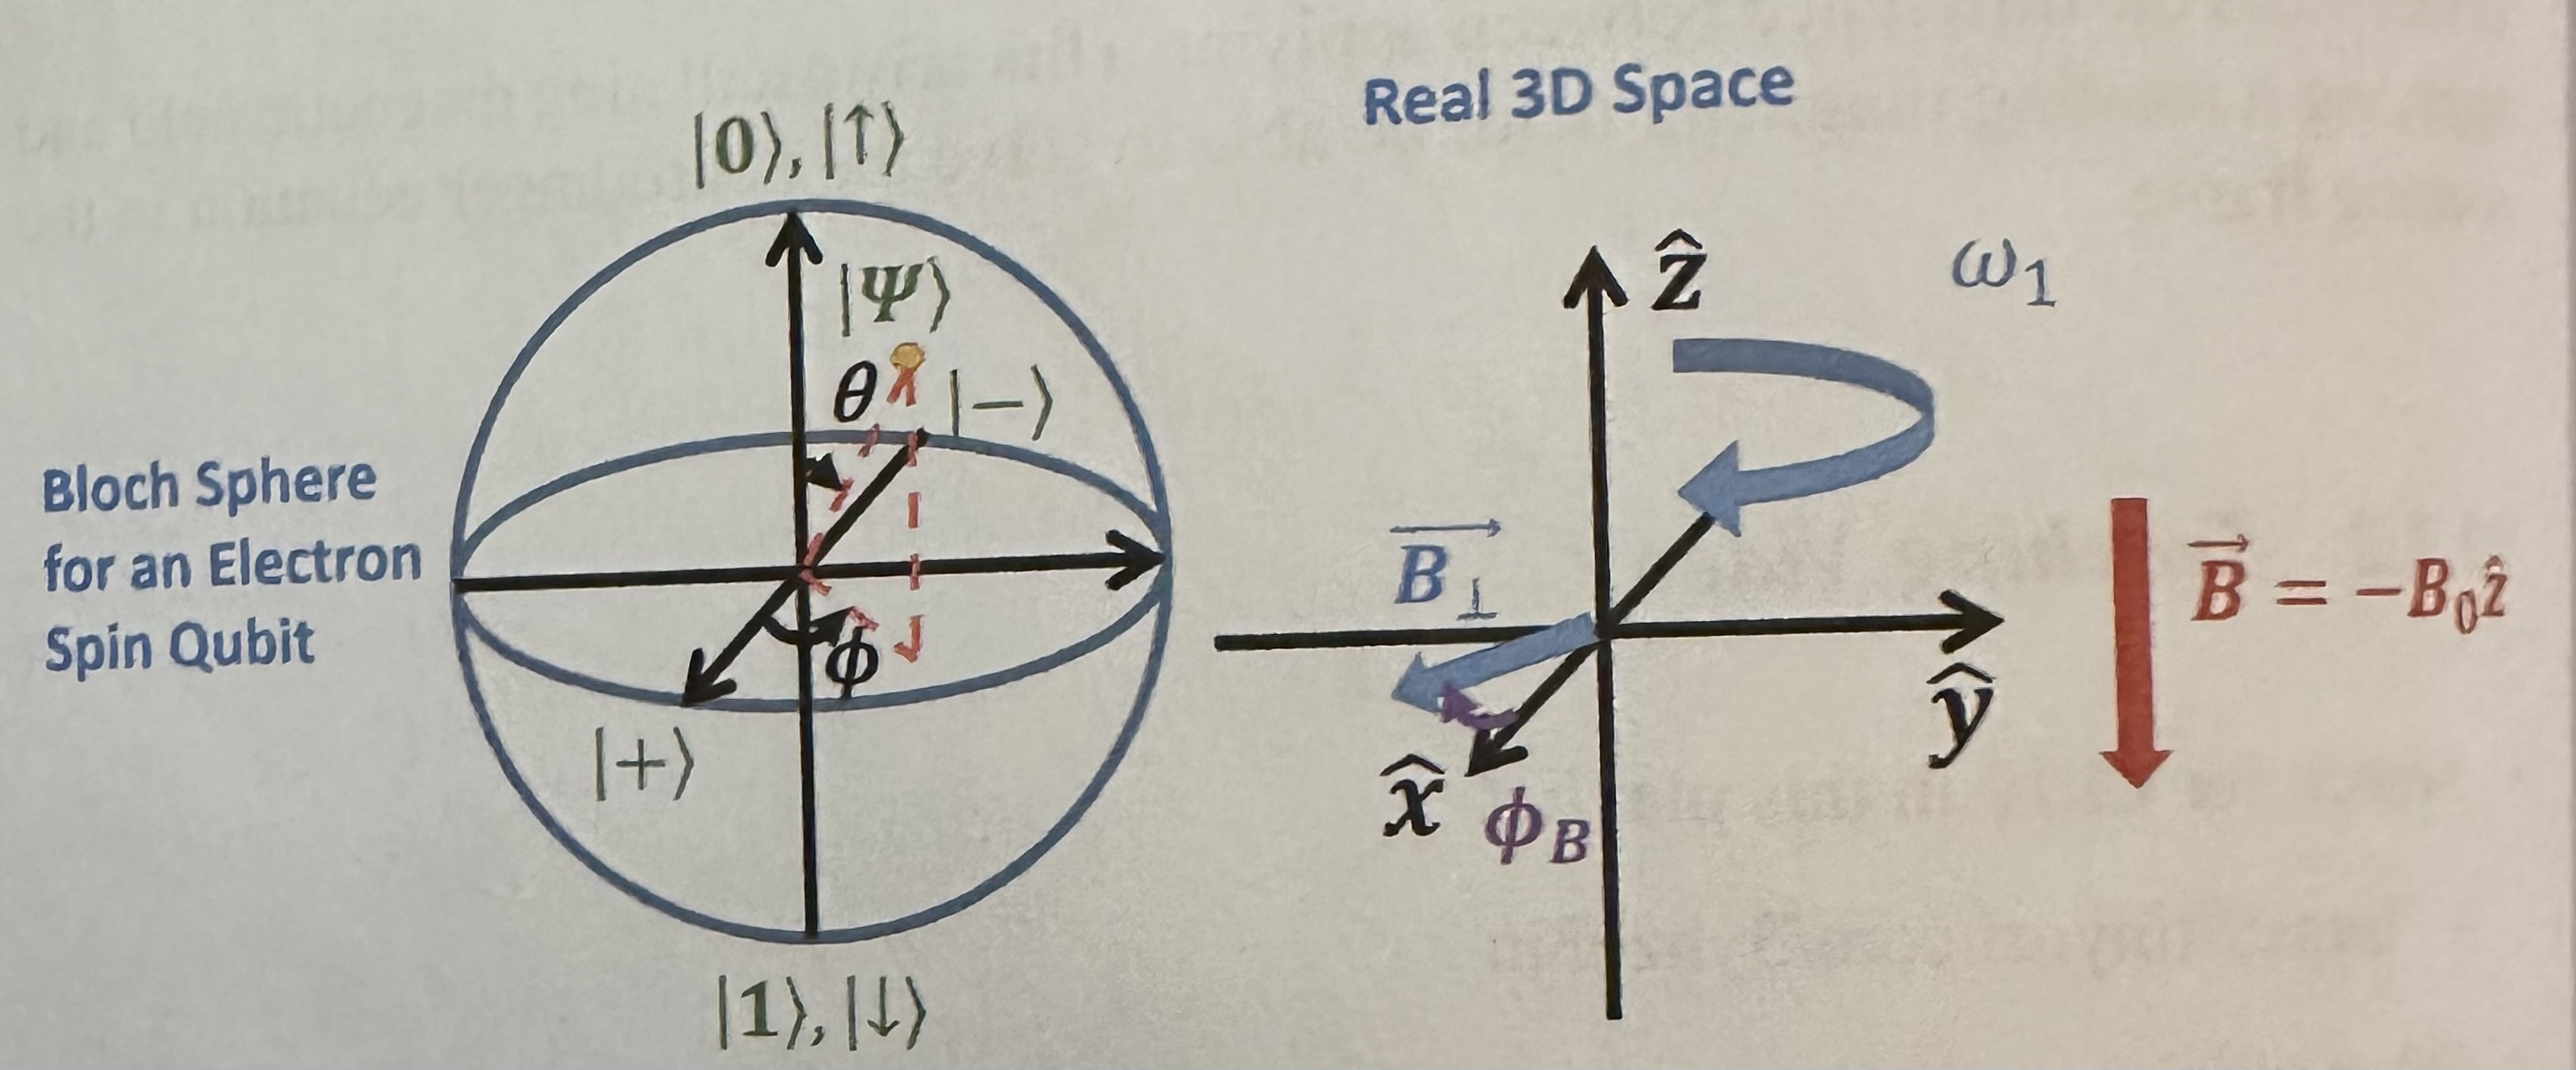
\includegraphics[scale=0.45]{Fig.10.1.jpeg}\\
\textbf{Fig. 10.1} The Bloch sphere representation of an electron spin qubit (left) and the real 3D space
coordinate system in which the directions of the external constant and rotating magnetic fields are  shown.
The rotating field has an angular frequency $\omega_1$ and an initial phase $\phi_B$. It rotates clockwise
when seeing from the top. \textit{Note that $\phi_B$ is measured in the clockwise direction}\\\\\\
\textbf{\large 10.3 Setting Up the Hamiltonian}\\\\
Therefore, the Hamiltonian is given by Eq. (9.3) as
\begin{align*}\label{eq 10.3}
    \boldsymbol{H}&=-\vec{B}\cdot\gamma\vec{S},\\
    &\approx(\frac{e}{m}\vec{S})\cdot\vec{B},\\
    &=\frac{e\hbar}{2m}(\boldsymbol{\sigma_x}\hat{x}+\boldsymbol{\sigma_y}\hat{y}+\boldsymbol{\sigma_z}\hat{z})\cdot(B_x\hat{x}+B_y\hat{y}+B_z\hat{z}),\\
    &=\frac{e\hbar}{2m}(\boldsymbol{\sigma_x}\: \boldsymbol{\sigma_y}\: \boldsymbol{\sigma_z})\begin{pmatrix}
        B_\bot\cos(\omega_1t+\phi_B)\\
        -B_\bot\sin(\omega_1t+\phi_B)\\ -B_0
    \end{pmatrix},\\
    &=\frac{e\hbar}{2m}B_\bot\cos(\omega_1t+\phi_B)\boldsymbol{\sigma_x}-\frac{e\hbar}{2m}
        B_0\bot\sin(\omega_1t+\phi_B)\boldsymbol{\sigma_y}-\frac{e\hbar}{2m}B_0\boldsymbol{\sigma_z},\\
        &=\frac{\hbar\varOmega_R}{2}\cos(\omega_1t+\phi_B)\boldsymbol{\sigma_x}-\frac{\hbar\varOmega_R}{2}\sin(\omega_1t+\phi_B)\boldsymbol{\sigma_y}
        -\frac{\hbar\omega_L}{2}\boldsymbol{\sigma_z},\\
        &=\boldsymbol{H_1}+\boldsymbol{H_0}.\tag{10.3}
\end{align*}
which is similar to how we derived Eq. (9.6). In line 2, we used the approximation of $g\approx-2$ (see Eqs.(7.8) and (7.9)).
It should also be noted that $e=1.6\times10^{-19}C>0$. In line 3, we used Eq. (9.2).
In line 4, Eq. (\ref{eq 10.2}) is used. In line 6, we used the definition of Larmor frequency in 
Eq. (8.11). Again, the Hamiltonian is separated into two parts. The first part is $\boldsymbol{H_0}=\frac{-e\hbar}{2m}B_0\boldsymbol{\sigma_z}$. This 
is the same as Eq. (8.4) due to the interaction between the vertical constant magnetic field and the
spin magnetic moment. But now $\boldsymbol{H_1}=\frac{e\hbar}{2m}B_\bot\cos(\omega_1t+\phi_B)\boldsymbol{\sigma_x}-\frac{e\hbar}{2m}B_\bot\sin(\omega_1t+\phi_B)\boldsymbol{\sigma_y}$
is due to the rotating field. We also defined a new quantity, $\Omega_R$, which is the \textbf{Rabi frequency}
\textit{in this particular experimental setup}, as
\begin{align*}\label{eq 10.4}
    \varOmega_R&=\frac{e}{m}B_\bot,\\
    &=-\gamma B_\bot, \tag{10.4}
\end{align*}
where in the second line we reintroduce the \textit{gyromagnetic ratio}, $\gamma$, to get an exact solution as 
$\frac{e}{m}$ is just an approximation of $\gamma$ when $g\approx-2$. Note that again $e>0$ and $\gamma<0$ for an
electron spin qubit.

It is also instructive to compare $\varOmega_R$ to $\omega_R$ due to the linearly oscillating magnetic
field in Eq.(9.32). Both of them are propertional to the amplitude of the field and the gyromagnetic
ratio. But $\omega_R$ has an extra $\frac{1}{2}$ as it is linearly oscillating. 

Now we will introduce two quantities, $\boldsymbol{\sigma^+}$ and $\boldsymbol{\sigma^-}$.
\begin{align*}\label{eq 10.5}
    \boldsymbol{\sigma^+}&=\boldsymbol{\sigma_x}+i\boldsymbol{\sigma_y},\\
    \boldsymbol{\sigma^-}&=\boldsymbol{\sigma_x}-i\boldsymbol{\sigma_y}.\tag{10.5}
\end{align*}

They are also \textit{proportional} to the \textbf{raising} and \textbf{lowering operators} of $\boldsymbol{\sigma_z}$
(see Problem 10.1). Let us inspect their matrix form.
\begin{align*}\label{eq 10.6}
    \boldsymbol{\sigma^+}&=\boldsymbol{\sigma_x}+i\boldsymbol{\sigma_y},\\
    &=\begin{pmatrix}
        0\ 1\\ 1\ 0
    \end{pmatrix}+i\begin{pmatrix}
        0& -i\\ i& 0
    \end{pmatrix}=
    \begin{pmatrix}
        0\ 2\\ 0\ 0
    \end{pmatrix}.\tag{10.6}
\end{align*}
\begin{align*}\label{eq 10.7}
    \boldsymbol{\sigma^-}&=\boldsymbol{\sigma_x}-i\boldsymbol{\sigma_y},\\
    &=\begin{pmatrix}
        0\ 1\\ 1\ 0
    \end{pmatrix}-i\begin{pmatrix}
        0& -i\\ i& 0
    \end{pmatrix}=
    \begin{pmatrix}
        0\ 0\\ 2\ 0
    \end{pmatrix}.\tag{10.7}
\end{align*}

Using Eq. (\ref{eq 10.5}), we can represent $\boldsymbol{\sigma_x}$ and $\boldsymbol{\sigma_y}$ 
in terms of $\boldsymbol{\sigma^+}$ and $\boldsymbol{\sigma^-}$.
\begin{align*}\label{eq 10.8}
    \boldsymbol{\sigma_x}=\frac{\boldsymbol{\sigma^+}+\boldsymbol{\sigma^-}}{2},\\
    \boldsymbol{\sigma_y}=\frac{\boldsymbol{\sigma^+}-\boldsymbol{\sigma^-}}{2i}.\tag{10.8}
\end{align*}
We now will substitute Eq. (\ref{eq 10.8}) into Eq. (\ref{eq 10.3}), and the interaction 
Hamiltonian becomes,
\begin{align*}\label{eq 10.9}
    \boldsymbol{H_1}=&\frac{\hbar\varOmega_R}{2}\cos(\omega_1t+\phi_B)\boldsymbol{\sigma_x}-\frac{\hbar\varOmega_R}{2}\sin(\omega_1t+\phi_B)\boldsymbol{\sigma_y},\\
    =&\frac{\hbar\varOmega_R}{4}[\cos(\omega_1t+\phi_B)(\boldsymbol{\sigma^+}+\boldsymbol{\sigma^-})
    -\sin(\omega_1t+\phi_B)(\boldsymbol{\sigma^+}-\boldsymbol{\sigma^-})/i],\\
    =&\frac{\hbar\varOmega_R}{4}[\cos(\omega_1t+\phi_B)(\boldsymbol{\sigma^+}+\boldsymbol{\sigma^-})
    +i\sin(\omega_1t+\phi_B)(\boldsymbol{\sigma^+}-\boldsymbol{\sigma^-})],\\
    =&\frac{\hbar\varOmega_R}{4}[\cos(\omega_1t+\phi_B)+i\sin(\omega_1t+\phi_B)\boldsymbol{\sigma^+}+(\cos{\omega_1t+\phi_B}\\
    &-i\sin{\omega_1t+\phi_B}\boldsymbol{\sigma^-}],\\
    =&\frac{\hbar\varOmega_R}{4}[\exp \{ i(\omega_1t+\phi_B) \} \boldsymbol{\sigma^+}+\exp \{ -i(\omega_1t+\phi_B) \} \boldsymbol{\sigma^-}]. \tag{10.9}
\end{align*}
where Eq. (\ref{eq 10.8}) was used in line 2. In line 5, we used the identities $e^{i\theta}=\cos\theta+i\sin\theta$ and
$e^{i\theta}=\cos\theta-i\sin\theta$.

The total Hamiltonian becomes,
\begin{align*}\label{eq 10.10}
    \boldsymbol{H}=&\boldsymbol{H_1}+\boldsymbol{H_0},\\
    =&\frac{\hbar\varOmega_R}{4}[\exp \{ i(\omega_1t+\phi_B) \} \boldsymbol{\sigma^+}\\
    &+\exp \{ -i(\omega_1t+\phi_B) \} \boldsymbol{\sigma^-}]-\frac{\hbar\omega_L}{2}\boldsymbol{\sigma_z},\tag{10.10}
\end{align*}\\\\\\
\textbf{\large 10.4 Transforming to Rotating Frame}\\\\
The Schr\"{o}dinger equation with the time-dependent Hamiltonian in Eq. (\ref{eq 10.10}) is
difficult to solve. Unlike the treatment in the previous chapter, we do NOT assume 
$\boldsymbol{H_1}$ to be a perturbation and we cannot used the perturbation theory (or Eq. (9.8)).
To solve this, we will work on the \textbf{rotating frame} which rotates together with the
rotating magnetic field $\vec{B_\bot}$ at a frequency of $\omega_1$. \textit{Note that this is \textbf{NOT} rotating at 
Larmor precession as in the case in Fig. 9.4}.

The Schr\"{o}dinger equation to be solved in the laboratory frame is,
\begin{equation}\label{eq 10.11}
    i\hbar\frac{\partial \ket{\psi}}{\partial t}=(\boldsymbol{H_0}+\boldsymbol{H_1})\ket{\psi}=\boldsymbol{H}\ket{\psi},\tag{10.11}
\end{equation}
with \bfit{H} given in Eq. (\ref{eq 10.10}). To solve it in the rotating frame, let us first find the
unitary transformation, \bfit{U}, that will rotate a state at the same rate and same direction as how 
$\vec{B_\bot}$ is rotating. This means that in this frame, we will see $\vec{B_\bot}$ as a constant rotating at 
$\omega_1$. We know that Larmor precession is due to $\boldsymbol{H_0}$, and the corresponding rotation matrix is given
by (see Eq. (4.9)),
\begin{align*}\label{eq 10.12}
    \boldsymbol{U_L}=&e^{-i\frac{\boldsymbol{H_0}t}{\hbar}},\\
    =&e^{-i\frac{-\hbar\omega_L\boldsymbol{\sigma_z}t}{2\hbar}},\\
    =&e^{i\frac{\omega_Lt}{2}\boldsymbol{\sigma_z}}.\tag{10.12}
\end{align*}

Note that the Larmor precession and the rotating field are both rotating clockwise
in this case. Therefore, the unitary matrix corresponding to \textit{rotating a state at}
$\omega_1$ must have the same form but with $\omega_L$ in the euqation. Therefore,
\begin{equation}\label{eq 10.13}
    \boldsymbol{U}=e^{i\frac{\omega_1t}{2}\boldsymbol{\sigma_z}}.\tag{10.13}
\end{equation}

If we are in the rotating frame, we should see the stationalry wavefunction \textit{in the laboratory
frame}, $\ket{\psi}$, rotating in the opposite direction. This is equivalent to applying
\bfit{U}$^\dagger$ to $\ket{\psi}$ in the laboratory frame if we want to describe it in the rotating
frame. Therefore, in the rotating frame, a stat $\ket{\psi}$ will become $\boldsymbol{U}^\dagger\ket{\psi}$.
We define $\boldsymbol{U_{RF}}=\boldsymbol{U}^\dagger$,
\begin{equation}\label{eq 10.14}
    \boldsymbol{U_{R F}}=\boldsymbol{U}^\dagger=e^{-i\frac{\omega_Lt}{2}\boldsymbol{\sigma_z}},\tag{10.14}
\end{equation}
The state $\ket{\psi}$ in the laboratory frame becomes $\ket{\psi}_{RF}$
though the following equation,
\begin{equation}\label{eq 10.15}
    \ket{\psi}_{RF}=\boldsymbol{U_{RF}}\ket{\psi}.\tag{10.15}
\end{equation}

we can also find the inverse of $\boldsymbol{U_{RF}}$ as,
\begin{equation}\label{eq 10.16}
    \boldsymbol{U}^\dagger_{\boldsymbol{RF}}=e^{i\frac{\omega_1t}{2}\boldsymbol{\sigma_z}},\tag{10.16}
\end{equation}

Therefore, \textbf{in the rotating frame}, the Schr\"{o}dinger equation becomes,
\begin{equation}\label{eq 10.17}
    i\hbar\frac{\partial \ket{\psi}_{RF}}{\partial t}=\boldsymbol{H_{RF}}\ket{\psi}_{RF},\tag{10.17}
\end{equation}
where $\boldsymbol{H_{RF}}$ is the total Hamiltonian in the rotating frame, We need to find 
$\boldsymbol{H_{RF}}$ but it is not straightforward. We cannot just apply $\boldsymbol{U_{RF}H}\boldsymbol{U}^\dagger_{\boldsymbol{RF}}$
to get $\boldsymbol{H_{RF}}$ because of the differential term on the left (as
$\boldsymbol{U_{RF}}\frac{\partial \ket{\psi}}{\partial t})\neq \frac{\partial(\boldsymbol{U_{RF}}\ket{\psi})}{\partial t})$.
We will show how to solve it in the next section.\\\\\\
\textbf{\large 10.5 Solving the Schr\"{o}dinger Equation}\\\\
Now, we need to find $\boldsymbol{H_{RF}}$. In this section, we will go through the details of the mathematics. After this section, readers are advised to read Sect. 10.7 in which 
canned eqautions can be used to speed up the process. We substitute Eq. (\ref{eq 10.15})
into the left-hand side of Eq. (\ref{eq 10.17}),
\begin{align*}\label{eq 10.18}
    i\hbar\frac{\partial \ket{\psi}_{RF}}{\partial t}=&i\hbar\frac{\partial}{\partial t}(\boldsymbol{U_{RF}}\ket{\psi}),\\
    =&i\hbar\frac{\partial\boldsymbol{U_{RF}}}{\partial t}\ket{\psi}+i\hbar\boldsymbol{U_{RF}}\frac{\partial \ket{\psi}}{\partial t},\\
    =&i\hbar\frac{\partial\boldsymbol{U_{RF}}}{\partial t}\ket{\psi}+\boldsymbol{U_{RF}H}\ket{\psi}, \tag{10.18}
\end{align*}
where we have use the \textit{chain rule} in line 2 and Eq. (\ref{eq 10.11}) in line 3. Since $\ket{\psi}=\boldsymbol{U}^\dagger_{\boldsymbol{RF}}\ket{\psi}_{RF}$
(inverse of Eq. (\ref{eq 10.15})), we continue to change Eq. (\ref{eq 10.18}) to,
\begin{align*}\label{eq 10.19}
    i\hbar\frac{\partial \ket{\psi}_{RF}}{\partial t}=&i\hbar\frac{\partial \boldsymbol{U_{RF}}}{\partial t}\boldsymbol{U}^\dagger_{\boldsymbol{RF}}\ket{\psi}_{RF}
    +\boldsymbol{U_{RF}H}\boldsymbol{U}^\dagger_{\boldsymbol{RF}}\ket{\psi}_{RF},\\
    =&\left(i\hbar\frac{\partial \boldsymbol{U_{RF}}}{\partial t}\boldsymbol{U}^\dagger_{\boldsymbol{RF}}+\boldsymbol{U_{RF}H}\boldsymbol{U}^\dagger_{\boldsymbol{RF}}\right)\ket{\psi}_{RF},\\
    =&\boldsymbol{H_{RF}}\ket{\psi}_{RF}. \tag{10.19}
\end{align*}

By using the trick above, we have successfully found that,
\begin{equation}\label{eq 10.20}
    \boldsymbol{H_{RF}}=i\hbar\frac{\partial \boldsymbol{U_{RF}}}{\partial t}\boldsymbol{U}^\dagger_{\boldsymbol{RF}}+\boldsymbol{U_{RF}H}\boldsymbol{U}^\dagger_{\boldsymbol{RF}}.\tag{10.20}
\end{equation}

Now, we will further expand $\boldsymbol{H_{RF}}$ to terms that can helps us solve the Schr\"{o}dinger equation.
Let us evaluate the first term on the right-hand side by substituting Eqs. (\ref{eq 10.14}) and (\ref{eq 10.16})
into Eq. (\ref{eq 10.20}).
\begin{align*}\label{eq 10.21}
    i\hbar\frac{\partial \boldsymbol{U_{RF}}}{\partial t}\boldsymbol{U}^\dagger_{\boldsymbol{RF}}=\ &i\hbar\frac{\partial}{\partial t}\left(e^{-i\frac{\omega_1t}{2}}\boldsymbol{\sigma_z}\right)e^{i\frac{\omega_1t}{2}}\boldsymbol{\sigma_z},\\
    =\ &i\hbar\left(-i\frac{\omega_1}{2}\boldsymbol{\sigma_z}e^{-i\frac{\omega_1t}{2}\boldsymbol{\sigma_z}}\right)e^{i\frac{\omega_1t}{2}\boldsymbol{\sigma_z}},\\
    =\ &\frac{\hbar\omega_1}{2}\boldsymbol{\sigma_z},\tag{10.21}
\end{align*}
where we performed derivative easily as $\boldsymbol{\sigma_z}$ is diagonal. Now consider the 
\textit{second term} on the right-hand side of Eq. (\ref{eq 10.20}). We substitute Eq. (\ref{eq 10.10})
and obtain,
\begin{align*}\label{eq 10.22}
    \boldsymbol{U_{RF}H}\boldsymbol{U}^\dagger_{\boldsymbol{RF}} =\ &\boldsymbol{U_{RF}}\bigg( \frac{\hbar\varOmega_R}{4}[\exp \{ i(\omega_1t+\phi_B) \} \boldsymbol{\sigma^+}\\
    &+\exp \{ -i(\omega_1t+\phi_B) \} \boldsymbol{\sigma^-}]-\frac{\hbar\omega_L}{2}\boldsymbol{\sigma_z}\bigg)\boldsymbol{U}^\dagger_{\boldsymbol{RF}},\\
    =\ &\frac{\hbar\varOmega_R}{4}\exp \{ i(\omega_1t+\phi_B) \} \boldsymbol{U_{RF}\sigma^+}\boldsymbol{U}^\dagger_{\boldsymbol{RF}}\\
    &+\frac{\hbar\varOmega_R}{4}\exp \{ -i(\omega_1t+\phi_B) \} \boldsymbol{U_{RF}\sigma^-}\boldsymbol{U}^\dagger_{\boldsymbol{RF}}\\
    &-\frac{\hbar\omega_L}{2}\boldsymbol{U_{RF}\sigma_z}\boldsymbol{U}^\dagger_{\boldsymbol{RF}},\tag{10.22}
\end{align*}

This is pretty daunting. But we can solve it term by term. Firstly, let us work on the last
term. This one is easy if we recognize that $\boldsymbol{U_{RF}}$ and $\boldsymbol{U}^\dagger_{\boldsymbol{RF}}$
are the exponentiations of $\boldsymbol{\sigma_z}$ (Eqs.(\ref{eq 10.14}) and (\ref{eq 10.16})) and, thus, it is diagoanl
(see Sect. 4.3.1 about the exponentiation of a diagonal matrix). Therefore, they commut
with $\boldsymbol{\sigma_z}\boldsymbol{U}^\dagger_{\boldsymbol{RF}}=\boldsymbol{U}^\dagger_{\boldsymbol{RF}}\boldsymbol{\sigma_z}$
and,
\begin{align*}\label{eq 10.23}
    -\frac{\hbar\omega_L}{2}\boldsymbol{U_{RF}\sigma_z}\boldsymbol{U}^\dagger_{\boldsymbol{RF}}=\ &
    -\frac{\hbar\omega_L}{2}e^{-i\frac{\omega_1t}{2}\boldsymbol{\sigma_z}}\boldsymbol{\sigma_z}e^{i\frac{\omega_1t}{2}\boldsymbol{\sigma_z}}\\
    =\ &-\frac{\hbar\omega_L}{2}\left(e^{-i\frac{\omega_1t}{2}\boldsymbol{\sigma_z}}e^{i\frac{\omega_1t}{2}\boldsymbol{\sigma_z}}\right)\boldsymbol{\sigma_z},\\
    =\ & -\frac{\hbar\omega_L}{2}\boldsymbol{\sigma_z}.\tag{10.23}
\end{align*}

To find the first and second term of Eq. (\ref{eq 10.22}), we need to find 
$\boldsymbol{U_{RF}\sigma^+}\boldsymbol{U}^\dagger_{\boldsymbol{RF}}$ and
$\boldsymbol{U_{RF}\sigma^-}\boldsymbol{U}^\dagger_{\boldsymbol{RF}}$.
It turns out that
\begin{align*}\label{eq 10.24}
    \boldsymbol{U_{RF}\sigma^+}\boldsymbol{U}^\dagger_{\boldsymbol{RF}}&=e^{-i\omega_1t}\boldsymbol{\sigma^+},\\
    \boldsymbol{U_{RF}\sigma^-}\boldsymbol{U}^\dagger_{\boldsymbol{RF}}&=e^{i\omega_1t}\boldsymbol{\sigma^-}.\tag{10.24}
\end{align*}
Let us prove the first one and try the second one in q problem.\\\\
\textbf{Example 10.1} Show that $\boldsymbol{U_{RF}\sigma^+}\boldsymbol{U}^\dagger_{\boldsymbol{RF}}=e^{-i\omega_1t}\boldsymbol{\sigma^+}$,

It is easy to show if we used their matrix form. Firstly, based on Eqs. (\ref{eq 10.14}) and (\ref{eq 10.16}),
\begin{align*}
    \boldsymbol{U_{RF}}&=e^{-i\frac{\omega_1t}{2}\boldsymbol{\sigma_z}}=\begin{pmatrix}
        e^{-i\frac{\omega_1t}{2}}&0\\0&e^{i\frac{\omega_1t}{2}}
    \end{pmatrix},\\
    \boldsymbol{U}^\dagger_{\boldsymbol{RF}}&=e^{i\frac{\omega_1t}{2}\boldsymbol{\sigma_z}}=\begin{pmatrix}
        e^{i\frac{\omega_1t}{2}}&0\\0&e^{-i\frac{\omega_1t}{2}}
    \end{pmatrix}.
\end{align*}

With Eq. (\ref{eq 10.6}), the left-hand side is,
\begin{align*}
      \boldsymbol{U_{RF}\sigma^+}\boldsymbol{U}^\dagger_{\boldsymbol{RF}}&=
      \begin{pmatrix}
        e^{-i\frac{\omega_1t}{2}}&0\\0&e^{i\frac{\omega_1t}{2}}
    \end{pmatrix}
    \begin{pmatrix}
        0\ 2\\ 0 \ 0
    \end{pmatrix}
    \begin{pmatrix}
        e^{i\frac{\omega_1t}{2}}&0\\0&e^{-i\frac{\omega_1t}{2}}
    \end{pmatrix},\\
    &=\begin{pmatrix}
        e^{-i\frac{\omega_1t}{2}}&0\\0&e^{i\frac{\omega_1t}{2}}
    \end{pmatrix}.\begin{pmatrix}
       0& 2e^{-i\frac{\omega_1t}{2}}\\0&0
    \end{pmatrix},\\
    &= \begin{pmatrix}
        0& 2e^{-i\omega_1t}\\0&0
    \end{pmatrix},\\
    &= e^{-i\omega_1t}\begin{pmatrix}
        0\ 2\\ 0\ 0
    \end{pmatrix},\\
    &= e^{-i\omega_1t}\boldsymbol{\sigma^+}.
\end{align*}
\hfill $\blacksquare$

Therefore, by substituting with Eqs. (\ref{eq 10.21}) and (\ref{eq 10.22}), Eq. (\ref{eq 10.20})
becomes,
\begin{align*}\label{eq 10.25}
    \boldsymbol{H_{RF}}=\ & i\hbar\frac{\partial \boldsymbol{U_{RF}}}{\partial t}\boldsymbol{U}^\dagger_{\boldsymbol{RF}}+\boldsymbol{U_{RF}H}\boldsymbol{U}^\dagger_{\boldsymbol{RF}},\\
    =\ &\frac{\hbar\omega_1}{2}\boldsymbol{\sigma_z}\\
    &+\frac{\hbar\varOmega}{4}\exp\{i(\omega_1t+\phi_B)\}\boldsymbol{U_{RF}\sigma^+}\boldsymbol{U}^\dagger_{\boldsymbol{RF}}\\
    &+\frac{\hbar\varOmega}{4}\exp\{-i(\omega_1t+\phi_B)\}\boldsymbol{U_{RF}\sigma^-}\boldsymbol{U}^\dagger_{\boldsymbol{RF}}\\
    &-\frac{\hbar\omega_L}{2}\boldsymbol{U_{RF}\sigma_z}\boldsymbol{U}^\dagger_{\boldsymbol{RF}}. \tag{10.25}
\end{align*}

We then further substitute with Eqs. (\ref{eq 10.23}) and (\ref{eq 10.24}), then
\begin{align*}\label{eq 10.26}
    \boldsymbol{H_{RF}}=\ &\frac{\hbar\omega_1}{2}\boldsymbol{\sigma_z}\\
    &+\frac{\hbar\varOmega_R}{4}\exp\{i(\omega_1t+\phi_B)\}e^{-i\omega_1t}\boldsymbol{\sigma^+}\\
    &+\frac{\hbar\varOmega_R}{4}\exp\{-i(\omega_1t+\phi_B)\}e^{i\omega_1t}\boldsymbol{\sigma^-}\\
    &-\frac{\hbar\omega_L}{2}\boldsymbol{\sigma_z},\\
    =\ &-\frac{\hbar(\omega_L-\omega_1)}{2}\boldsymbol{\sigma_z}+\frac{\hbar\varOmega_R}{4}\bigg(e^{i\phi_B}\boldsymbol{\sigma^+}
    +e^{-i\phi_B}\boldsymbol{\sigma^-}\bigg),\\
    =\ &-\frac{\hbar\varDelta }{2}\boldsymbol{\sigma_z}+\frac{\hbar\varOmega_R}{4}\bigg(e^{i\phi_B}\boldsymbol{\sigma^+}+
    +e^{-i\phi_B}\boldsymbol{\sigma^-}\bigg).\tag{10.26}
\end{align*}
where we have introduced the definition of \textbf{detuning}, $\varDelta=\omega_L-\omega_1$, which is the 
\textit{difference between the Larmor frequency and the rotating frame frequency}. In some literature, it is 
defined as $\omega_1-\omega_L$. Now, let us now replace $\boldsymbol{\sigma^+}$ and $\boldsymbol{\sigma^-}$
by $\boldsymbol{\sigma_x}$ and $\boldsymbol{\sigma_y}$ using Eq. (\ref{eq 10.5}).
\begin{align*}\label{eq 10.27}
    \boldsymbol{H_{RF}}&=-\frac{\hbar\varDelta }{2}\boldsymbol{\sigma_z}+\frac{\hbar\varOmega_R}{4}\bigg(e^{i\phi_B}(\boldsymbol{\sigma_x}+i\boldsymbol{\sigma_y})
    +e^{-i\phi_B}(\boldsymbol{\sigma_x}-i\boldsymbol{\sigma_y})\bigg),\\
    &=-\frac{\hbar\varDelta }{2}\boldsymbol{\sigma_z}+\frac{\hbar\varOmega_R}{4}(2\cos\phi_B\boldsymbol{\sigma_x}-2\sin\phi_B\boldsymbol{\sigma_y}),\\
    &=-\frac{\hbar\varDelta }{2}\boldsymbol{\sigma_z}+\frac{\hbar\varOmega_R}{2}(\cos\phi_B\boldsymbol{\sigma_x}-\sin\phi_B\boldsymbol{\sigma_y}),\\
    &=\frac{\hbar}{2}\begin{pmatrix}
        \boldsymbol{\sigma_x} \ \boldsymbol{\sigma_y} \ \boldsymbol{\sigma_z}
    \end{pmatrix}\cdot
    \begin{pmatrix}
        \varOmega_R\cos\phi_B\\
        -\varOmega_R\sin\phi_B\\
        -\varDelta 
    \end{pmatrix},\\
    &=\frac{\hbar}{2}\vec{\boldsymbol{\sigma}}\cdot\vec{\varOmega_R}=\frac{\hbar}{2}\vec{\varOmega_R}\cdot\vec{\boldsymbol{\sigma}},\tag{10.27}
\end{align*}
where in line 2, we used the identities $e^{i\theta}=\cos\theta+i\sin\theta$ and
$e^{-i\theta}=\cos\theta-i\sin\theta$. In line 5, we defined the \textbf{angular frequency vector},
$\vec{\varOmega_R}$, as
\begin{equation}\label{eq 10.28}
    \vec{\varOmega_R}= \begin{pmatrix}
        \varOmega_R\cos\phi_B\\
        -\varOmega_R\sin\phi_B\\
        -\varDelta 
    \end{pmatrix}.\tag{10.28}
\end{equation}

We have gone through a lot of derivations and we probably forget what we are
doing. Our goal is to solve the Schr/"{o}dinger equation in the rotating frame, which is
Eq. (\ref{eq 10.17}). We finally express $\boldsymbol{H_P{RF}}$ in the rotating frame as in
Eq. (\ref{eq 10.27}). Note that now $\boldsymbol{H_{RF}}$ in Eq. (\ref{eq 10.27}) is 
\textbf{time dependent} and we can solve it easily. The Schr/"{o}dinger equation now becomes
\begin{equation}\label{eq 10.29}
    i\hbar\frac{\partial \ket{\psi}_{RF}}{\partial t}=\frac{\hbar}{2}\vec{\varOmega_R}\cdot\vec{\boldsymbol{\sigma}}\ket{\psi}_{RF}. \tag{10.29}
\end{equation}

While $\boldsymbol{H_{RF}}$ is a constant, it is not diagoanl. We can solve it using its matrix form
using the method in Sect. 4.3.2. However, we will not solve it here. We will use our intuition.\\\\\\
\textbf{\large 10.6 Intuitive Understanding of the Solution}\\\\
Let us recall the Hamiltonian of a constant magnetic field pointing downward is
given in Eq. (8.4). By using Eq. (8.11), it becomes
\begin{align*}\label{eq 10.30}
    \boldsymbol{H}&=-B_0\frac{e\hbar}{2m}\boldsymbol{\sigma_z},\\
    &= -\frac{\hbar\omega_L}{2}\boldsymbol{\sigma_z},\\
    &=\frac{\hbar}{2}\begin{pmatrix}
        \boldsymbol{\sigma_x}\ \boldsymbol{\sigma_y}\ \boldsymbol{\sigma_z} 
    \end{pmatrix}\cdot
    \begin{pmatrix}
        0\\0\\ -\omega_L
    \end{pmatrix}. \tag{10.30}
\end{align*}

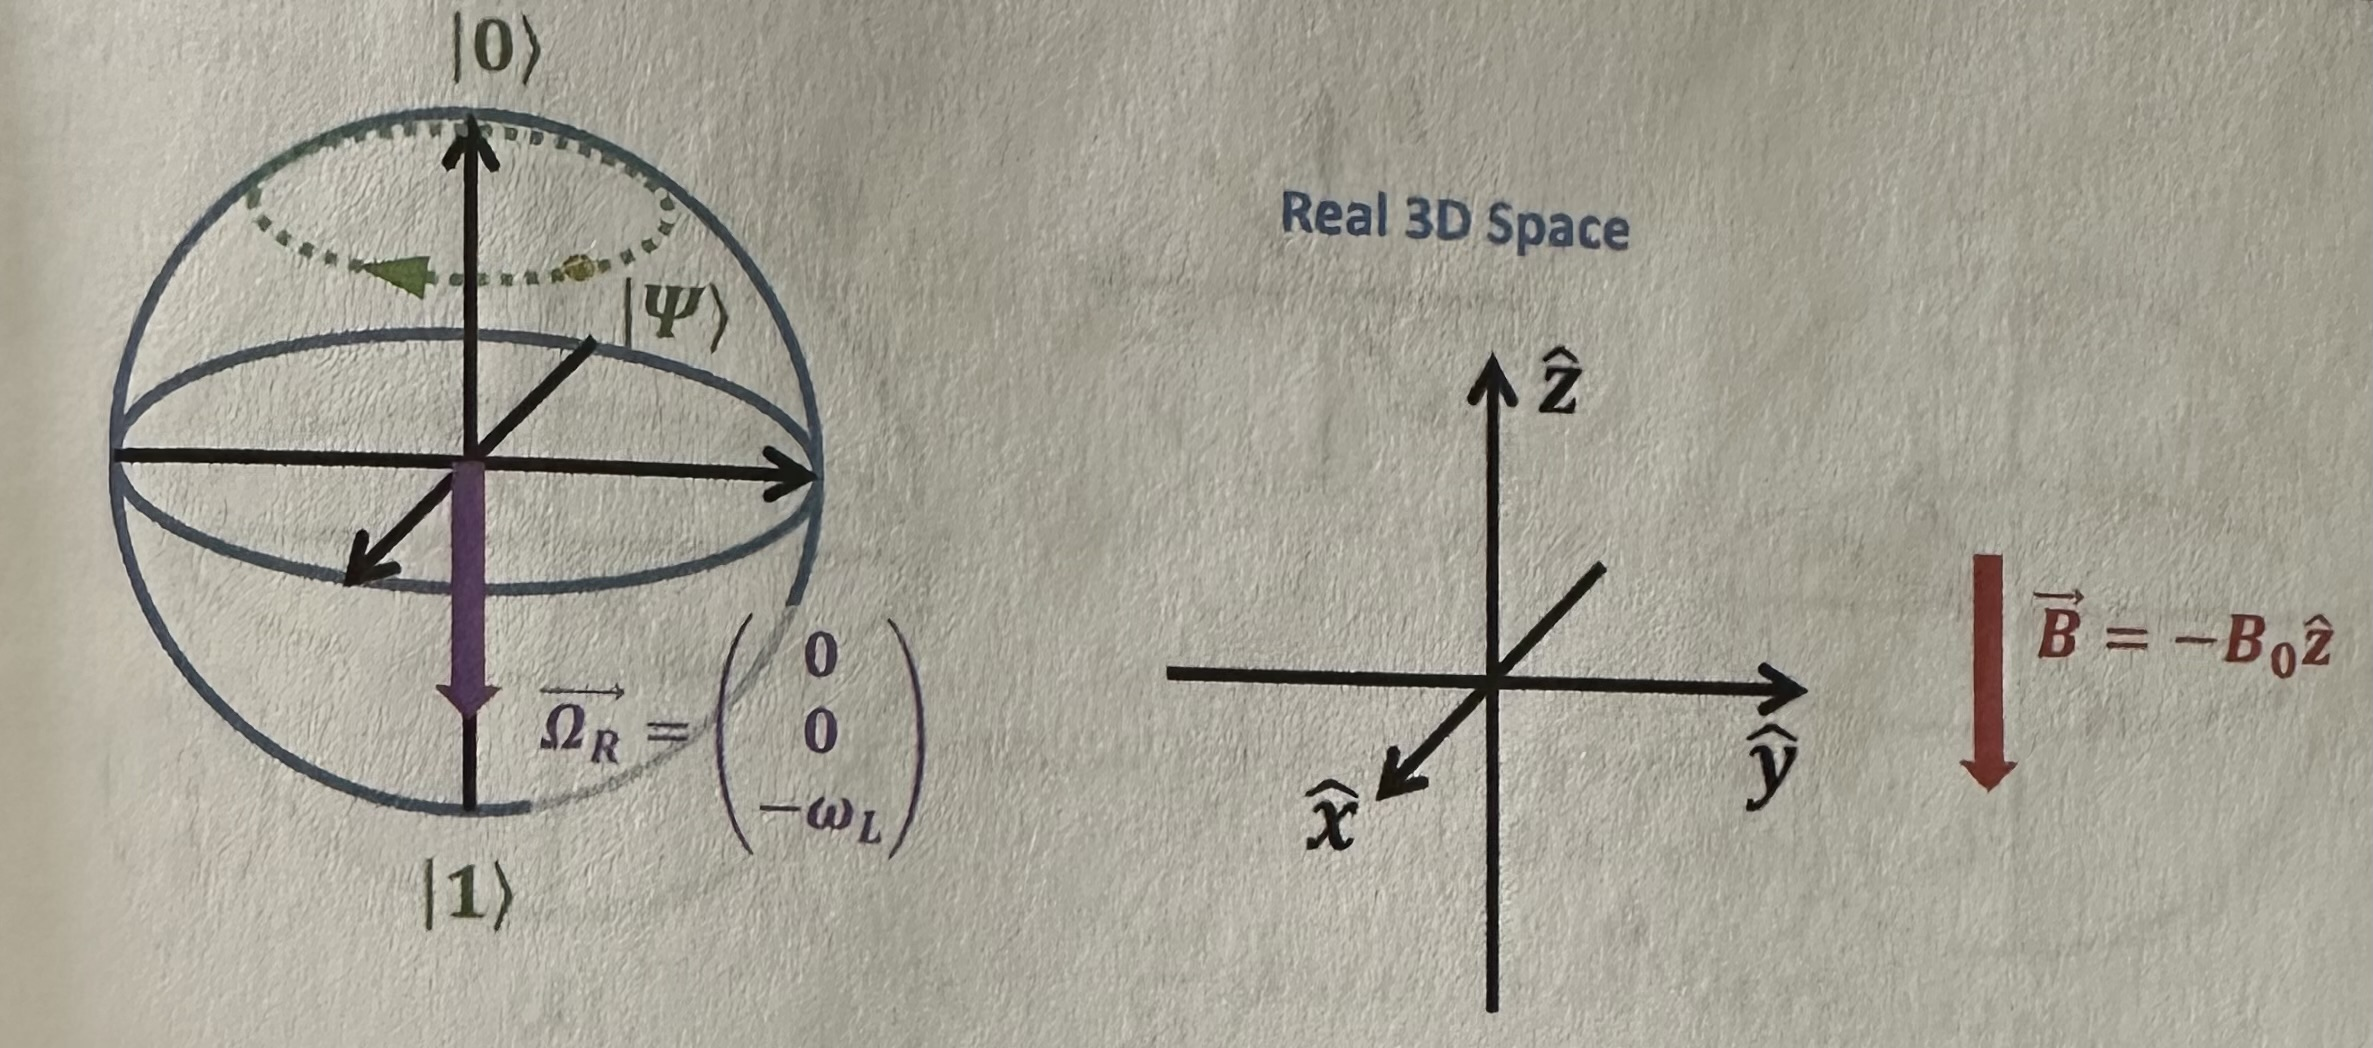
\includegraphics[scale=0.5]{Fig.10.2.jpeg}\\
\textbf{Fig.10.2} Redraw of Fig. 8.1 with the angular velocity vector and the precession of state
$\ket{\psi}$. Left: The Bloch sphere representation of an electron spin eubit. Right: The real 3D space coordinate
system in which the direction of the external magnetic field is show. Note that it is still in the laboratory frame\\

We see that it is just a special case of Eq. (\ref{eq 10.27}) with $\vec{\varOmega_R}=\begin{pmatrix}
    0\\0\\-\omega_L
\end{pmatrix}$ and $\varDelta=\omega_L$ (i.e., it is in the laboratory frame). Figure 10.2 shows
the direction of $\vec{\varOmega_R}$. Based on this figure, we see that Larmor precession can be understood as the rotation
about $\vec{\varOmega_R}$ (using right-hand-rule). Moreover, \textit{the magnitude of $\vec{\varOmega_R}$ determines the precession frequency}.

We therefore can guess that precession will occur about $\vec{\varOmega_R}$ for Eq. (\ref{eq 10.29}). At the left
of Fig. 10.3, it showss the precession aobut a general angular velocity vector.
The right of the figure shows the precession about $\vec{\varOmega_R}=\begin{pmatrix}
    \varOmega_R\cos0\\ -\varOmega_R\sin0\\0
\end{pmatrix}= \begin{pmatrix}
    \varOmega_R\\0\\0
\end{pmatrix}$. This is the case when $\varPhi_B=0$. And it is easy to understand becuase we are in the 
rotating frame at $\omega_1$. If $\varPhi_B=0$, then the rotating magnetic field always points at 
$\hat{x^\prime}$.

Therefore, if we set an appropriated initial phase for the rotating frame, $\varPhi_B=0$, an
appropriate $\varOmega_R$, and an appropriate $\omega_1$ (thus the detuning), we can control the
direction and the magnitude of $\vec{\varOmega_R}$. This then determines the rotation frequency and
the rotation direction of a quantum state! The rotation frequency, or the \textbf{generalized Rabi frequency},
$\varOmega_R^\prime$, is 
\begin{equation}\label{eq 10.31}
    \varOmega_R^\prime=|\vec{\varOmega_R}|=\sqrt{\varOmega_R^2+\varDelta^2}.\tag{10.31}
\end{equation}
\textbf{And we need to remind ourselves that we are working in the rotating frame} to get the picture in Fig. 10.3.\\

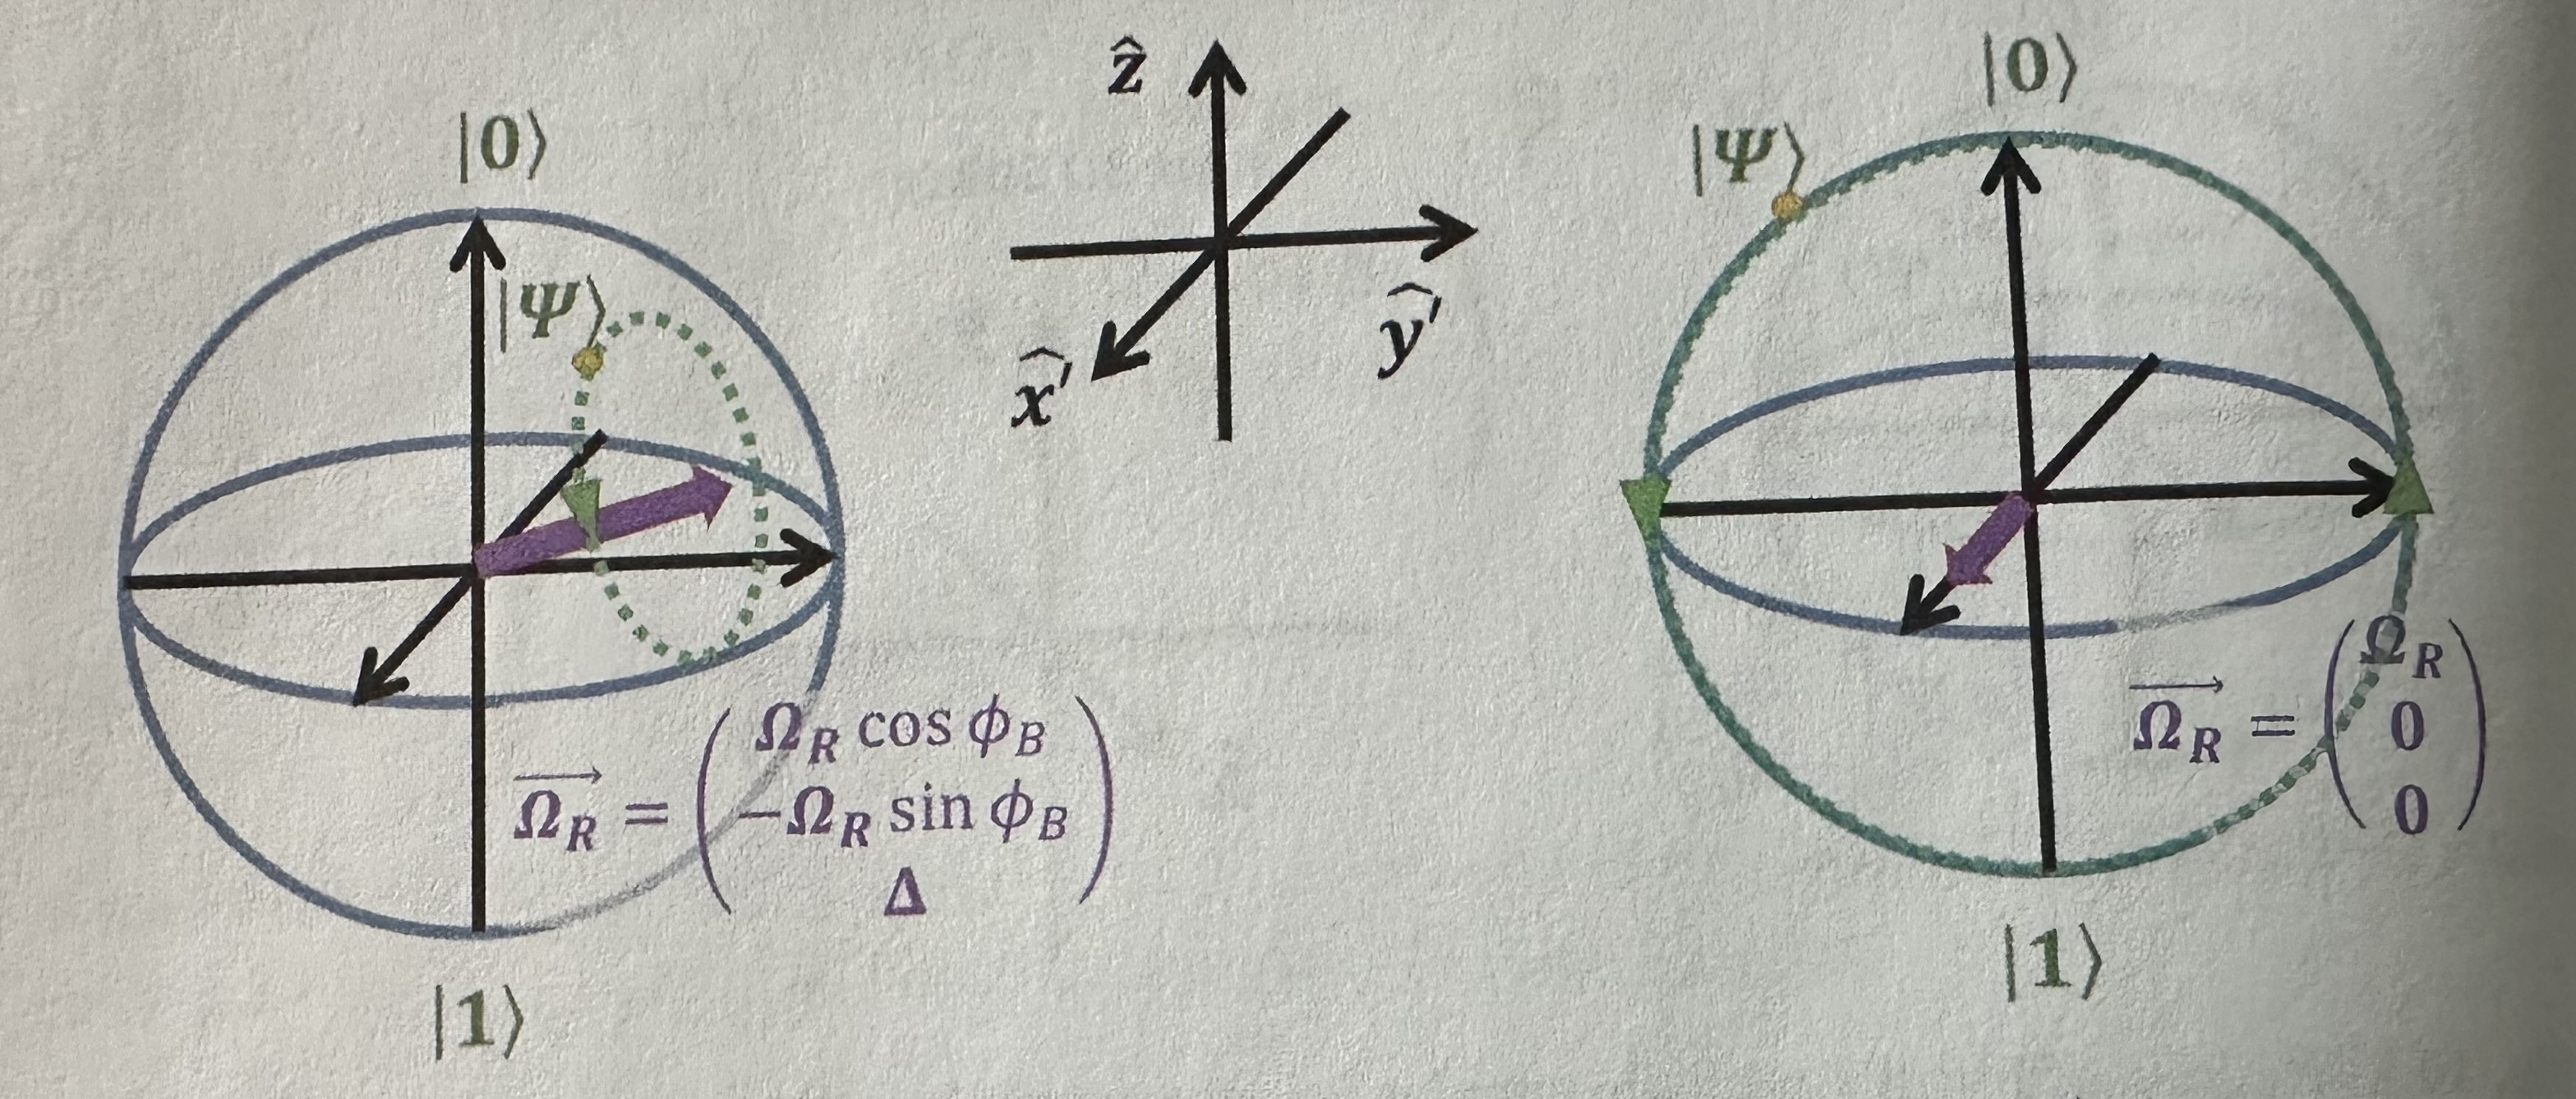
\includegraphics[scale=0.5]{Fig. 10.3.jpeg}\\
\textbf{Fig. 10.3} Illustration of prevession about a general angular velocity vector, $\vec{\varOmega_R}$
(left), and about a special vector pointing at the $\hat{x}$ direction (right). Note that this in the \textbf{rotating frame}\\\\\\
\textbf{\large 10.7 Another Method to Perform Rotating Frame Transformation}\\\\
In Eq. (\ref{eq 10.20}), we showed the relationship between $\boldsymbol{H_{RF}}$ and $\boldsymbol{H}$. We see that it has
two terms. The first term is $i\hbar\frac{\partial \boldsymbol{U_{RF}}}{\partial t}\boldsymbol{U}^\dagger_{\boldsymbol{RF}}$.
This term has nothing to do with $\boldsymbol{H}$ and it is always $\frac{\hbar\omega_L}{2}\boldsymbol{\sigma_z}$ (Eq.(\ref{eq 10.21})).
Together with the natural precession, they form the final detuning term.

For the second term, it is the transformation of \bfit{H}. If \bfit{H} is a linear combination of
$\boldsymbol{\sigma_x}, \boldsymbol{\sigma_y}$ and $\boldsymbol{\sigma_z}$, one may obtain their transformation
easily by using the following identities:
\begin{align*}\label{eq 10.32}
    \boldsymbol{U_{RF}\sigma_x}\boldsymbol{U}^\dagger_{\boldsymbol{RF}}&=\cos\omega_1t\boldsymbol{\sigma_x}+\sin\omega_1t\boldsymbol{\sigma_y},\tag{10.32}\\
    \boldsymbol{U_{RF}\sigma_y}\boldsymbol{U}^\dagger_{\boldsymbol{RF}}&=\cos\omega_1t\boldsymbol{\sigma_y}-\sin\omega_1t\boldsymbol{\sigma_x},\tag{10.33}\\
    \boldsymbol{U_{RF}\sigma_z}\boldsymbol{U}^\dagger_{\boldsymbol{RF}}&=\boldsymbol{\sigma_z},\tag{10.34}\\
    \boldsymbol{U_{RF}\sigma^+}\boldsymbol{U}^\dagger_{\boldsymbol{RF}}&=e^{-i\omega_1t}\boldsymbol{\sigma^+},\tag{10.35}\\
    \boldsymbol{U_{RF}\sigma^-}\boldsymbol{U}^\dagger_{\boldsymbol{RF}}&=e^{i\omega_1t}\boldsymbol{\sigma^-}.\tag{10.36}
\end{align*}

For example, we may jsut apply them to Eq. (\ref{eq 10.3}) to obtain the results. Of course, we need to make sure to include
$i\hbar\frac{\partial \boldsymbol{U_{RF}}}{\partial t}\boldsymbol{U}^\dagger_{\boldsymbol{RF}}=\frac{\hbar\omega_1}{2}\boldsymbol{\sigma_z}$.\\\\
\textbf{Example 10.2} Derive Eq. (\ref{eq 10.27}) from Eq. (\ref{eq 10.3}) using Eq. (\ref{eq 10.20}) and Eqs.(10.32)-(10.34).

From Eq. (\ref{eq 10.3}), we have
\begin{equation}\label{eq 10.37}
    \boldsymbol{H}=\frac{\hbar\varOmega_R}{2}\cos(\omega_1t+\phi_B)\boldsymbol{\sigma_x}-\frac{\hbar\varOmega_R}{2}\sin(\omega_1t+\phi_B)\boldsymbol{\sigma_y}
    -\frac{\hbar\omega_L}{2}\boldsymbol{\sigma_z}.\tag{10.37}
\end{equation}
Therefore,
\begin{align*}\label{eq 10.38}
    \boldsymbol{H_{RF}}=\ &i\hbar\frac{\partial \boldsymbol{U_{RF}}}{\partial t}\boldsymbol{U}^\dagger_{\boldsymbol{RF}}+
    \boldsymbol{U_{RF}H}\boldsymbol{U}^\dagger_{\boldsymbol{RF}},\\
    =\ &\frac{\hbar\omega_1}{2}\boldsymbol{\sigma_z}+\boldsymbol{U_{RF}}\bigg[\frac{\hbar\varOmega_R}{2}\cos(\omega_1t+\phi_B)\boldsymbol{\sigma_x}\\
    &-\frac{\hbar\varOmega_R}{2}\sin(\omega_1t+\phi_B)\boldsymbol{\sigma_y}-\frac{\hbar\omega_L}{2}\boldsymbol{\sigma_z}\bigg]\boldsymbol{U}^\dagger_{\boldsymbol{RF}},\\
    =\ &-\frac{\hbar\varDelta}{2}\boldsymbol{\sigma_z}+\frac{\hbar\varOmega_R}{2}\cos(\omega_1t+\phi_B)
    \boldsymbol{U_{RF}\sigma_x}\boldsymbol{U}^\dagger_{\boldsymbol{RF}}\\
    &-\frac{\hbar\varOmega_R}{2}\sin(\omega_1t+\phi_B)\boldsymbol{U_{RF}\sigma_y}\boldsymbol{U}^\dagger_{\boldsymbol{RF}}. \tag{10.38}
\end{align*}
where we have used Eq. (10.34) and combined the $\boldsymbol{\sigma_z}$ terms as a detuning term with
$\varDelta=\omega_L-\omega_1$. We then use the trigonometric identities and Eqs.(\ref{eq 10.20}) and (\ref{eq 10.32}).
For example,
\begin{align*}\label{eq 10.39}
    &\cos(\omega_1t+\phi_B) \boldsymbol{U_{RF}\sigma_x}\boldsymbol{U}^\dagger_{\boldsymbol{RF}}\\
    =&\cos(\omega_1t+\phi_B)(\cos\omega_1t\boldsymbol{\sigma_x}+\sin\omega_1t\boldsymbol{\sigma_y}),\\
    =&\cos(\omega_1t+\phi_B)\cos\omega_1t\boldsymbol{\sigma_x}+
    \cos(\omega_1t+\phi_B)\sin\omega_1t\boldsymbol{\sigma_y}. \tag{10.39}
\end{align*}
Similarly,
\begin{align*}\label{eq 10.40}
    &\sin(\omega_1t+\phi_B) \boldsymbol{U_{RF}\sigma_y}\boldsymbol{U}^\dagger_{\boldsymbol{RF}}\\
    =&\sin(\omega_1t+\phi_B)(\cos\omega_1t\boldsymbol{\sigma_y}-\sin\omega_1t\boldsymbol{\sigma_x}),\\
    =&\sin(\omega_1t+\phi_B)\cos\omega_1t\boldsymbol{\sigma_y}-
    \sin(\omega_1t+\phi_B)\sin\omega_1t\boldsymbol{\sigma_x}. \tag{10.40}
\end{align*}
Therefore, substituting Eqs.(\ref{eq 10.39}) and (\ref{eq 10.40}) into Eq. (\ref{eq 10.38}) and using trigonometric identities, we obtain
\begin{align*}\label{eq 10.41}
    \boldsymbol{H_{RF}}=\ &-\frac{\hbar\varDelta}{2}\boldsymbol{\sigma_z}+
    \frac{\hbar\varOmega_R}{2}\cos(\omega_1t+\phi_B)\boldsymbol{U_{RF}\sigma_x}\boldsymbol{U}^\dagger_{\boldsymbol{RF}}\\
    &-\frac{\hbar\varOmega_R}{2}\sin(\omega_1t+\phi_B)\boldsymbol{U_{RF}\sigma_y}\boldsymbol{U}^\dagger_{\boldsymbol{RF}},\\
    =\ &-\frac{\hbar\varDelta}{2}\boldsymbol{\sigma_z}+\frac{\hbar\varOmega_R}{2}(\cos\phi_B\boldsymbol{\sigma_x}-\sin\phi_B\boldsymbol{\sigma_y}).\tag{10.41}
\end{align*}
This is the same as Eq. (\ref{eq 10.27}). \hfill $\blacksquare$\\\\
\textbf{\large 10.8 Summary}\\\\
In this chapter, we study the change of an electron spin qubit under a constant vertical magentic field and 
a rotating magnetic field on the $\hat{x}-\hat{y}$ plane. We work on the rotating frame of 
the rotating field to simplify the problem. Under the rotating frame, the Hamiltonian becomes time-independent.
The effective external magnetic field becomes a constant megnetic field pointing in a certain
direction with a certain magnitude determined by the phase, frequency, and magnitude of 
the rotating magnetic field and the magnitude of the DC field. This then determines
the generalized Rabi frequency of a qubit state and its rotation direction. The picture we see in this chapter
will be reused in other types of qubits such as the superconducting qubits.\\\\\\
\textbf{\large Problems}\\\\
\textbf{10.1 Raising and Lowering Operators}
Sometimes $\boldsymbol{\sigma^+}$ and $\boldsymbol{\sigma^-}$ are defined as,
\begin{align*}
    \boldsymbol{\sigma^+}=\frac{\boldsymbol{\sigma_x}+i\boldsymbol{\sigma_y}}{2},\\
    \boldsymbol{\sigma^-}=\frac{\boldsymbol{\sigma_x}-i\boldsymbol{\sigma_y}}{2},\tag{10.42}
\end{align*}
and they are called the raising and lowering operators of $\boldsymbol{\sigma_z}$.

Find their matrix representations. Then apply them to $\ket{0}=\begin{pmatrix}
    1\\0
\end{pmatrix}$ and $\ket{1}=\begin{pmatrix}
    0\\1
\end{pmatrix}$. What do you see? You find that $\ket{0}=\boldsymbol{\sigma^+}\ket{1}$.
So what does it raise? It does not raise $\ket{0}$ and $\ket{1}$. Instead, it raises
the lower eigenvalue eigenvector of $\boldsymbol{\sigma_z}$ (i.e., $\ket{1}$ with eigenvalue
of $-1$) to the higher eigenvalue eigenvector of $\boldsymbol{\sigma_z}$ (i.e., $\ket{0}$
with eigenvalue of 1). We need to pay attention to be ambiguities.\\\\
\textbf{10.2 Rotating Frame Equations}\\
Prove Eqs.(10.32)-(10.34).\\\\
\textbf{10.3 Rotating Frame}\\
We skipped some steps in Example 10.2. Please show all steps.
\end{document}